%
% General structure for the revdetua class:
%
\documentclass[portugues,final]{revdetua}
\usepackage[portuguese]{babel}
\usepackage{listingsutf8}
\usepackage[utf8]{inputenc}
\usepackage[T1]{fontenc}
\usepackage{graphicx}
\usepackage{hyperref}
\usepackage{wrapfig}
\usepackage{float}
\usepackage{color}
\usepackage{amsmath}
\usepackage{eurosym}
%
% Valid options are:
%
%   longpaper --------- \part and \tableofcontents defined
%   shortpaper -------- \part and \tableofcontents not defined (default)
%
%   english ----------- main language is English (default)
%   portugues --------- main language is Portuguese
%
%   draft ------------- draft version
%   final ------------- final version (default)
%
%   times ------------- use times (postscript) fonts for text
%
%   mirror ------------ prints a mirror image of the paper (with dvips)
%
%   visiblelabels ----- \SL, \SN, \SP, \EL, \EN, etc. defined
%   invisiblelabels --- \SL, \SN, \SP, \EL, \EN, etc. not defined (default)
%
% Note: the final version should use the times fonts
% Note: the really final version should also use the mirror option
%


\begin{document}

% Note: the month must be in Portuguese

\title{\textbf{Bank Marketing}\\ Exploração de Dados \\Universidade de Aveiro}
\author{Diogo Silva 60337, Eduardo Sousa 68633}
\maketitle
\begin{resumo} % Note: in Portuguese
Este relatório descreve detalhadamente o processo que foi feito para analisar o data set Bank Marketing.
O processo inclui desde técnicas usadas, estratégias e até mesmo comparação de desempenho entre elas.
\end{resumo}

%\begin{palavraschave} % Note: in Portuguese (optional)
%\end{palavraschave}
\section{Geral}

Os dados que vão ser utilizados para este trabalho estão disponíveis em:
\url{https://archive.ics.uci.edu/ml/datasets/Bank+Marketing}

\subsection{Descrição das operações efetuadas}

Note-se que as operações listadas podem não ter sido aplicadas sobre os dados para todos os algoritmos, por exemplo, discretização não é necessária em Support Vector Machines, no entanto é necessária em Naive Bayes (sendo que na descrição do algoritmo é referido a operação efetuada sobre os dados).

\subsubsection{Enumeração}


Desenvolvimento - Esta operação foi efectuada sobre todos os algoritmos, sendo que foi desenvolvida através de um ficheiro PYTHON colocado na pasta src/data com o nome “transform\_data.py” sendo que o script vê todos os atributos que são strings e transforma pela ordem pedida pelo utilizador em números.\\

Lógica - Este método é necessário para todos os algoritmos devido ao facto de determinados atributos serem texto, como por exemplo, o atributo ‘month’ que pode assumir os valores (jan, feb, mar, ..., nov', dec) passa a assumir os valores 0, 1, 2, ..., 10, 11). O tratamento de texto durante o processamento de um algoritmo é algo pesado, enquanto efetuar a transformação do texto em inteiros antes do algoritmo não tem qualquer implicação.
Todos os atributos no dataset que eram categóricos com texto, passam a usar inteiros.\\
Ou seja, os atributos: job, marital, education, default, housing, loan, contact, month, day\_of\_week, poutcome.

\subsubsection{Discretização}

Este método consiste em tornar um dado atributo que pertence a um domínio contínuo num domínio discreto, porque dados algoritmos só podem trabalhar sobre dados em domínio discreto. Sendo que em vez de ter um atributo que assume qualquer valor de 0 a 10, passa apenas a assumir determinados valores nesse intervalo, por exemplo, passa a assumir apenas os valores inteiros (e.g. em vez de 0.45 passa-se a ter 0, e em vez de 0.55 passa-se a ter 1).

\subsubsection{Normalização - Feature Scaling}

Os dados vão ser normalizados não porque se tem o mesmo atributo em escalas diferentes (e.g. um valor estar em metros e o outro em milhas) mas porque se tem atributos que variam entre 0 e 10 e outros a variar entre 0 e 10000, para algoritmos que minimizam uma dada função de custo (e.g. SVM) e se os atributos estiverem normalizados, o algoritmo converge muito mais rápido.
A normalização que vai ser aplicada é a seguinte: 
\begin{center}{${X} = \frac{X - Xmin}{Xmax - Xmin}$}
\end{center}

Sendo que qualquer atributo passa a ter valores entre 0 e 1.

\subsubsection{Cross Validation}

Foi aplicado o método K-fold de forma a evitar erros na análise de cada algoritmos, sendo que é tirada uma porção do dataset para testes e a restante para treino, sendo que é efectuada esta divisão várias vezes durante este método.

\section{Descrição de operações para avaliar os algoritmos}

Desenvolvimento - Esta operação foi efectuada sobre todos os algoritmos, sendo que foi desenvolvida através de uma função MATLAB/Octave colocado na pasta src com o nome “fmeasure.m” sendo que recebe o class set esperado e o class set calculado, devolvendo o “accuracy”, “recall”, “precision” e “f-measure”. Permitindo assim tirar todas as conclusões necessárias.\\

Por norma “accuracy” chega para efectuar uma medição de acerto de um dado algoritmo, no entanto quando se trata de um caso de “Skewed classes” (quando existe muitos mais exemplos que pertencem a uma classe do que a outra), como é o caso, no dataset que vamos operar existe 36548 registos que pertencem a classe 0 e 4640 que pertencem a classe 1, estamos perante uma situação em que a classe positiva contém apenas 12\% do dataset, o que se torna dificil de avaliar usando apenas a fórmula “accuracy”.
Sendo assim para medir o desempenho de um dado algoritmo vai ser usado “F-measure” de forma a evitar este problema.

\section{Descrição dos métodos de classificação}

\subsection{K-Nearest Neighbors (KNN)}

\subsubsection{Teoria}

KNN é um algoritmo que permite efetuar classificação ou regressão sobre um data set, utilizando os k exemplos de treino mais próximos do valor para prever a classe ou valor da variável.\\

O algoritmo KNN durante a fase de treino limita-se a guardar os dados de treino, visto que depois para classificar um objeto terá de o inserir no espaço amostral e verificar quais são os k exemplos de treino mais próximos para prever qual a classe que deverá atribuir.\\

A distância pode ser calculada de diferentes formas, como por exemplo distância Euclidiana, distância de Manhattan, distância de Chebyshev, distância de Minkowski. A maneira como se calcula a distância vai ser um dos fatores mais importantes para o bom funcionamento, visto que se pode escolher um método de calcular a distância que favoreça mais uma feature do que outra. Além de se utilizar o melhor método para se calcular a distância, também se deve perceber se os k vizinhos mais próximos devem contribuir todos da mesma forma para a classificação, ou seja, se os k vizinhos contribuem uniformemente ou devemos atribuir um maior peso aos vizinhos que estejam mais próximos, ou seja, quando se estiver a calcular o peso desse vizinho na classificação do objeto deve-se dar um maior peso aos vizinhos mais perto do objeto.\\

Deve-se ter em conta que o número de vizinhos deve ser ímpar, para que não exista empate entre as distâncias calculadas. Deve-se também ter em conta que o número de vizinhos não deve ser múltiplo do número de classes presentes no data set.\\

\subsubsection{Desenvolvimento}

No desenvolvimento deste algoritmo utilizou-se o Octave, sendo o algoritmo todo desenvolvido pelos autores. Todos os passos do algoritmo foram vectorizados para que demora-se o mínimo de tempo possível a correr.\\

O algoritmo corre todas as distâncias implementadas, sendo elas:

\begin{itemize}
	\item Distância Euclidiana
	\item Distância Chebyshev
	\item Distância Manhattan
	\item Distância Minkowski
\end{itemize}

Estas distâncias foram utilizadas de duas formas, ou seja, após o calculo das distâncias é possível selecionar a classe fazendo a contagem do número de vizinhos em cada classe e a classe que tivesse mais vizinhos era a classe que era atribuída. A outra forma utilizada foi a de contar os vizinhos baseados na sua distância, ou seja, caso um vizinho esteja mais próximo irá influenciar mais para a contagem da classe a que pertence e um vizinho que esteja mais afastado irá contribuir menos.\\

\subsubsection{Desenvolvimento - Distância Euclidiana}

A distância Euclidiana é dada pela seguinte formula:\\

D (p, q) := $\sqrt{(q_1 - p_1)^2 + (q_2 - p_2)^2 + ... + (q_n - p_n)^2}$\\

\subsubsection{Desenvolvimento - Distância Chebyshev}

A distância Chebyshev é dada pela seguinte formula:\\

D (p, q) := $max_i(|p_i - q_i|)$\\

\subsubsection{Desenvolvimento - Distância Manhattan}

A distância Manhattan é dada pela seguinte formula:\\

D (p, q) := $\sum_{i=1}^{n}|p_i - q_i|$\\

\subsubsection{Desenvolvimento - Distância Minkowski}

A distância Minkowski é dada pela seguinte formula:\\

D (p, q) := $(\sum_{i=1}^{n}(|p_i - q_i|)^p)^{1/p}$\\

\subsubsection{Desenvolvimento - Análise do Desempenho}

De forma a determinar qual a melhor forma de cálculo de distância, o algoritmo foi testado utilizando diferentes porções do data set obtendo-se depois o valor médio para cada valor de K selecionado.\\

\begin{figure}[H]
\centerline{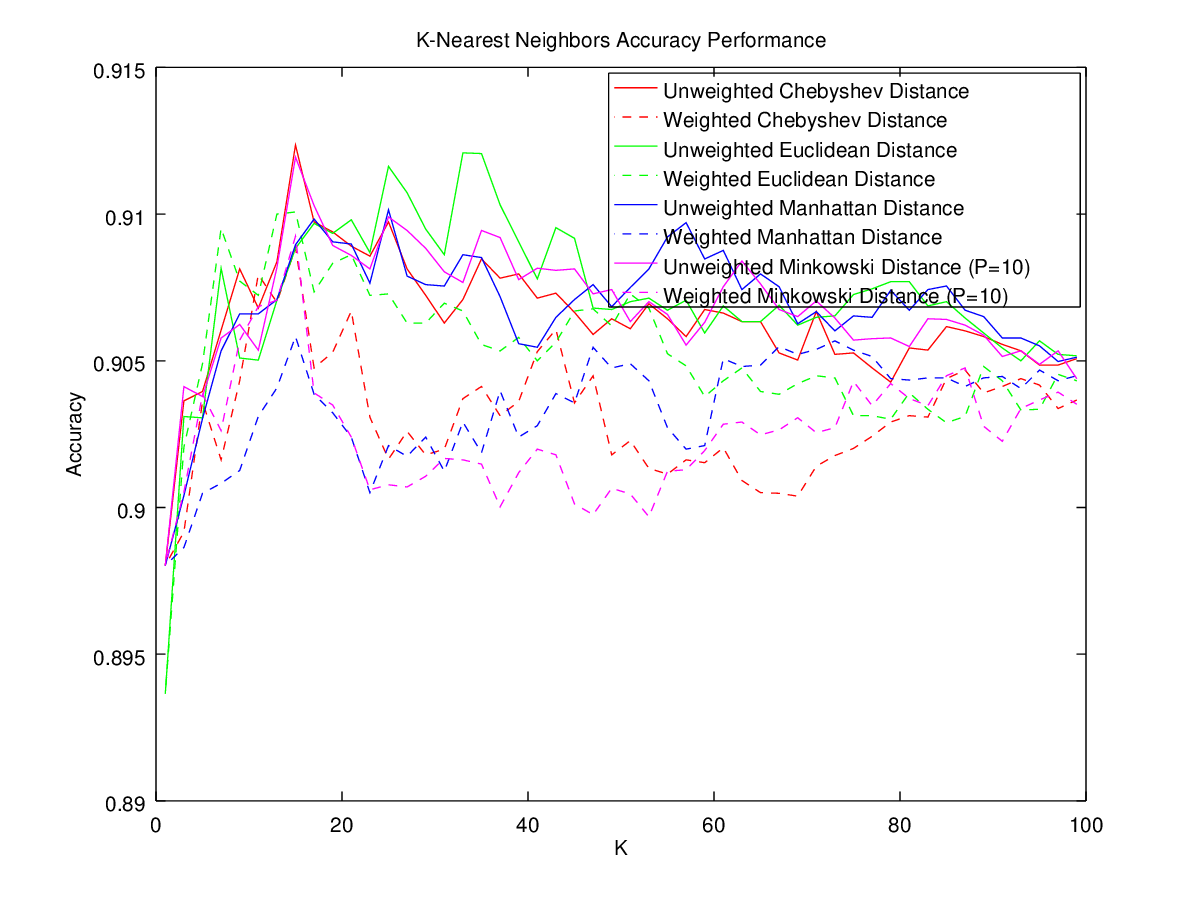
\includegraphics[width=230pt]{images/knn_graph_accuracy.png}}
\caption{Accuracy do K-Nearest Neighbors}
\label{img:complete}
\end{figure}

Embora possa parecer que o algoritmo segundo tenha uma Accuracy muito boa, esta não é um fator relevante, visto que o data set não tem percentagem igual de dados para cada classe.\\

\begin{figure}[H]
\centerline{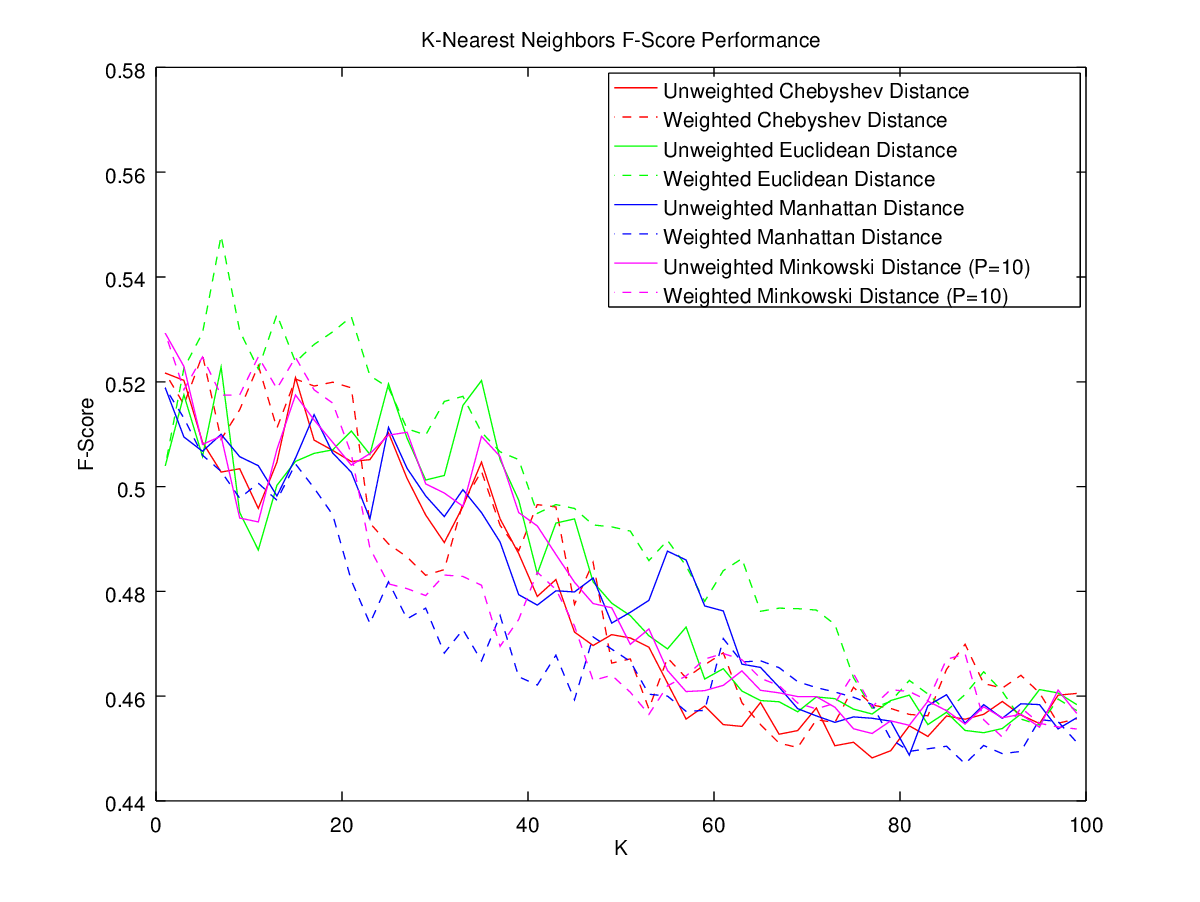
\includegraphics[width=230pt]{images/knn_graph_f-score.png}}
\caption{F-Score do K-Nearest Neighbors}
\label{img:complete}
\end{figure}

O F-Score não demonstra bons resultados, o que nos leva a crer que este algoritmo não seja o melhor para classificar este data set.\\

\begin{figure}[H]
\centerline{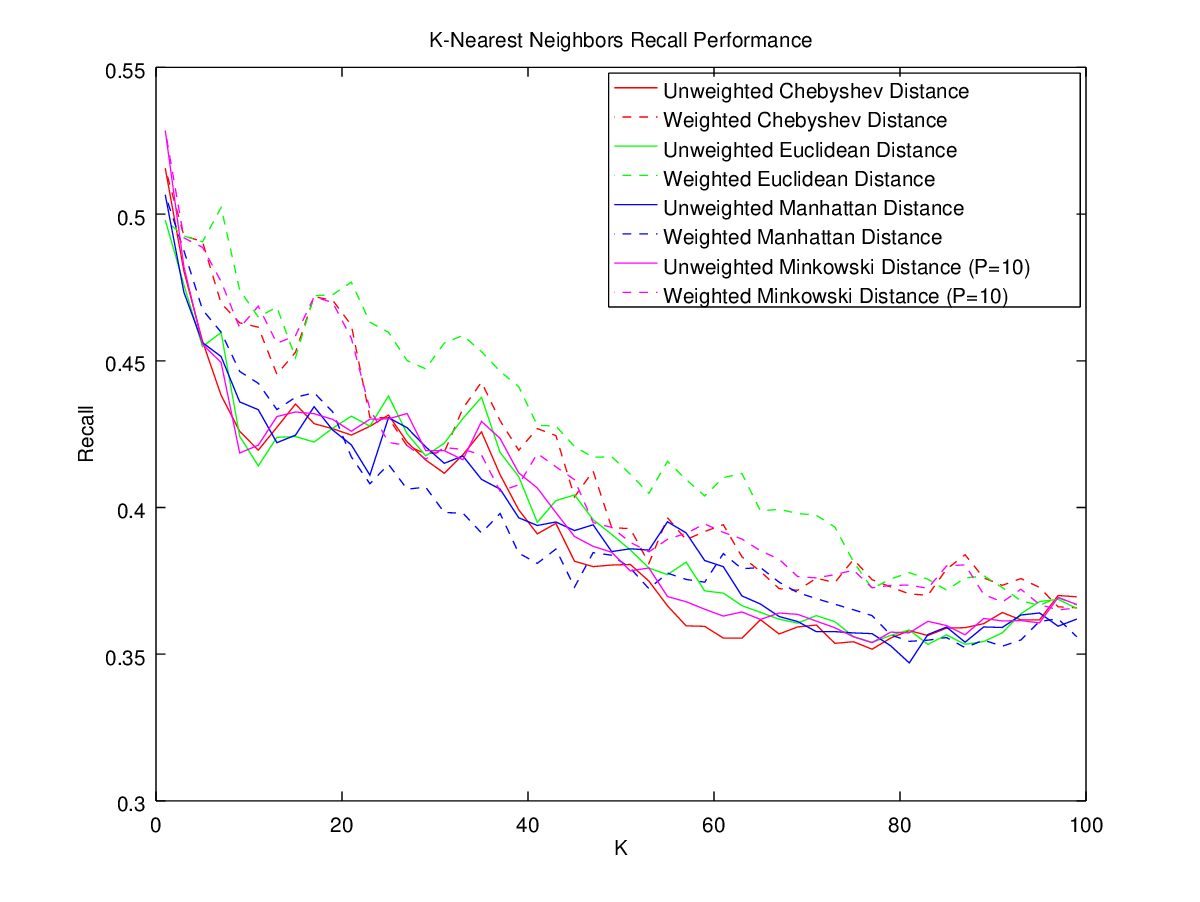
\includegraphics[width=230pt]{images/knn_graph_recall.png}}
\caption{Recall do K-Nearest Neighbors}
\label{img:complete}
\end{figure}

O Recall também não mostra bons resultados, visto que o valor mais alto ronda os 0.52.

Bibliografia consultada:\\
\url{https://en.wikipedia.org/wiki/K-nearest_neighbors_algorithm}\\
\url{http://scikit-learn.org/stable/modules/neighbors.html}

\subsubsection{Conclusão}

O fator mais importante neste problema é o Recall, sendo que o banco pretende saber se um determinado cliente tem maior tendência a subscrever a prazo ou não. É possível verificar nos gráficos acima que as melhores formas de calcular a distância entre os vizinhos que são as não uniformes (weighted), ou seja, onde consideramos que um vizinho mais próximo tem maior influência na escolha da classe, têm melhores resultados tanto no F-Score como no Recall, que são os fatores mais importantes neste problema.\\

\subsection{Support Vector Machine (SVM)}

\subsubsection{Teoria}
SVM é um algoritmo que permite efetuar classificação ou regressão sobre determinados dados, mais precisamente permite criar um “hiperplano” sobre N dimensões, neste caso, vamos ter 17 dimensões que são a quantidade de atributos (como são 17 dimensões não é visível num gráfico 2D ou 3D, sendo que seja provável que se aplique PCA para tornar visível o resultado do algoritmo graficamente).\\

Este algoritmo também é conhecido por “Maximum Margin Classifier” devido ao criar um plano de N dimensões tentar deixar a margem máxima (e equivalente) entre classes.\\

O algoritmo começa por: (1) Calcular os pesos relativos a cada atributo; (2) Calcula os valores de saída para os novos pesos; (3) Calcula a função de custo; (4) Volta ao passo 1 enquanto a função de custo continuar a decrescer.\\

Em situações em que as funções não são linearmente separáveis aplica-se um kernel de forma a criar funções não lineares que representem as necessidades.\\

Para o nosso caso como temos apenas 2 classes distintas não é necessário aplicar “one-agaisnt-all”.\\

Bibliografia usada:\\
\url{https://www.csie.ntu.edu.tw/~cjlin/libsvm/} - Biblioteca que vai ser usada em Octave\\
\url{https://www.youtube.com/watch?v=pkQyhSyP2QU&list=PLnnr1O8OWc6Zpr_yeQCPizmMbXpmsHXyx} - Coursera Course “Machine Learning” (SVM related videos)\\
\url{https://en.wikipedia.org/wiki/Support_vector_machine} - Conceitos foram pesquisados na Wikipedia, nos vídeos de youtube referidos acima e nos slides teóricos

\subsubsection{Desenvolvimento - Biblioteca/Software usado}
Inicialmente estava-se a usar Octave para fazer o desenvolvimento do SVM com a biblioteca LIBSVM.\\
LIBSVM: \url{https://www.csie.ntu.edu.tw/~cjlin/libsvm/}\\
No entanto notou-se que esta biblioteca não está completamente optimizada quando comparada com a biblioteca fornecida pelo MATLAB fitcsvm (no pacote stats), sendo que a biblioteca do MATLAB permite fazer a normalização dos valores adequada usando apenas um argumento no fitcsvm, como também permite definir o KernelScale em “auto” que significa que parâmetros como gamma e sigma do kernel RBF (por exemplo) são minimizados automaticamente para encontrar os melhores valores de desempenho.\\
Para além disso ainda permite definir a probabilidade de cada classe (uma optimização fornecida pelo fitcsvm) sendo que se fez a mean(TrainY) para a probabilidade da classe 0 ('no', classe mais provável) e $1 - mean(TrainY)$ para a classe 1 ('yes', classe menos provavel).

Sendo que a opção final foi de usar o MATLAB para desenvolver SVM. 

\subsubsection{Desenvolvimento - Análise da PCA}

Inicialmente foi pensado usar PCA para permitir a visualização dos 20 atributos, sendo que se transformava esses 20 atributos em 2 atributos que são os atributos correlacionados entre si, como se fosse dois novos atributos (componentes).

\begin{figure}[H]
\centerline{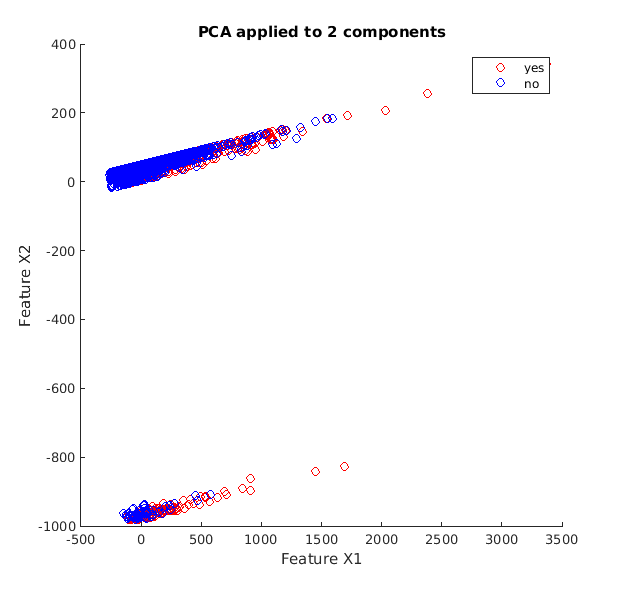
\includegraphics[width=230pt]{images/svm_pca.png}}
\caption{Resultado da PCA de 20 atributos para 2 componentes}
\label{img:complete}
\end{figure}

É possível verificar que existe classes nos dois ramos que foram separados, sendo que o ideal seria estar uma classe num ramo e outra noutro, ou pelo menos serem faceis de identificar as classes, o que significa que existe atributos que não colaboram muito para o cálculo da classe. Sendo que PCA não ajudou relativamente a visualização dos 20 atributos, tendo que se optar por fazer um estudo sobre as métricas de desempenho (accuracy, f-measure, recall, precision).

\subsubsection{Desenvolvimento - Estratégia adoptada}

Para o desenvolvimento do SVM usando as bibliotecas de MATLAB utilizou-se a seguinte sequência de passos:
\begin{enumerate}
\item Y = not(data(:, end)); Tornar a classe menos provável, a classe com o valor 1 sendo que o recall e o precision consideram que a classe menos provável é a classe 1 e a mais provável pertence a classe 0, sendo que na fórmula de cada um contém os True Positives em conta e não os True Negatives.
\item Normalizar os dados entre 0 e 1; $Xnorm = (X - repmat(minX, lX, 1)) ./ repmat(rangeX, lX, 1); $\\Encontra-se nas linhas 46 a 49 do script svmmain.m. Esta normalização vai permitir o SVM convergir mais rapidamente e até obter melhores valores devido ao conceito de kernel ter a distância entre os valores (basicamente vamos estar a normalizar as distâncias como consequência, o que é bom).
\item Obter os sets de Treino e de Teste usando cross validation, mais especificamente usou-se K-Fold devido a não se querer qualquer relação entre o Treino e o Teste. Cross-validation foi realizado na função 'splitset.m'.
\item Treinar os parametros do SVM recorrendo ao fitcsvm.
\item Obter os resultados do SVM para o set de Teste usando predict.
\item Calcular o desempenho do algoritmo e fazer a média para o K-Fold.
\end{enumerate}

\subsubsection{Desenvolvimento - Pré-análise}

Sendo que 10\% do dataset pertence a uma classe e 90\% pertence a outra classe, estamos num caso de 'Skewed Classes' sendo que existe a necessidade de recorrer a outra medidas que não 'accuracy' porque esta não leva em conta as classes em minoria, se eu desenvolver um algoritmo estático que diga que um exemplo pertence sempre a classe maioritaria, vou obter um 'accurary' de 90\%, no entanto o algoritmo não é muito bom porque nunca detecta casos da outra classe que são os mais importantes.\\

Tendo em conta o contexto real, no dataset pretende-se saber se um dado cliente vai subscrever a um depósito a termo ou não, sendo que a classe 1 corresponde ao cliente subscrever e classe 0 a não subscrever.\\

O banco tem todo o interesse de notificar todos os clientes que têm tendencia a subscrever um deposito a termo de novas ofertas sendo que é mais importante a medida de 'recall' do que 'precision'. O 'recall' serve para saber qual a percentagem de acerto dos casos em que a classe era 1 e que o algoritmo conseguiu detectar como da classe 1, ou seja, quanto maior o recall, maior é a probabilidade de conseguir atingir os clientes pretendidos.\\

Por outro lado, menos importante, o 'precision' que indica da percentagem dos clientes que o algoritmo detectou como pertencerem a classe 1 e que realmente eram dessa classe, ou seja, se o 'precision' for baixo vai acontecer que o banco vai estar a notificar pessoas que não eram supostas de novas ofertas.\\

No entanto, o 'recall' é mais importante que o 'precision' porque mais vale notificar pessoas a mais e atingir as que se pretende do que notificar a menos e não atingir as que se pretende.

\subsubsection{Desenvolvimento - Análise de Desempenho}

Para calcular o melhor desempenho do SVM sobre o dataset decidiu-se variar os parametros de entrada de cada Kernel. Sendo que nesta parte o MATLAB facilita um pouco fornecendo o parâmetro KernelScaling que permite variar um Kernel na sua totalidade.\\

\begin{figure}[H]
\centerline{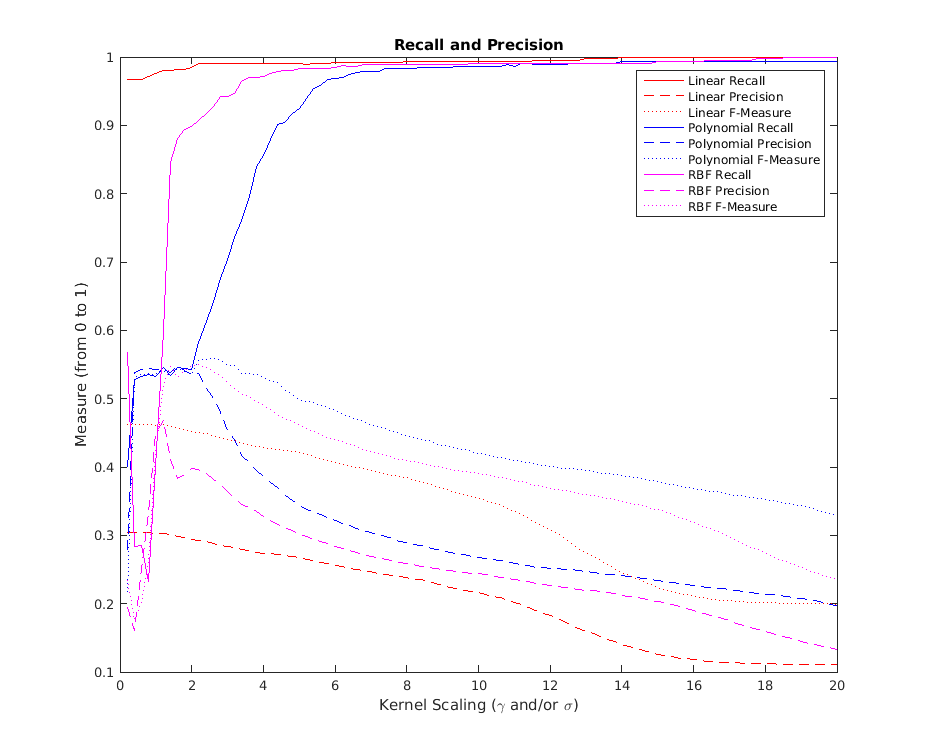
\includegraphics[width=290pt]{images/svm_recall_precision.png}}
\caption{Precision, Recall e F-Measure para cada algoritmo}
\label{img:complete}
\end{figure}


O gráfico anterior mostra que é possível atingir 'recall's bastante altos facilmente, que é o que se pretende, no entanto já que é possível obter recall bastante alto, vai-se também tentar optimizar a 'precision' o máximo possível sem que o 'recall' tenha muitas implicações.\\

SVM Linear - É possível verificar que com SVM linear é possível obter um 'recall' de ~0.97 e um 'precision' de ~0.3 (sendo esta a melhor situação para o SVM linear), sendo que o melhor f-measure para este caso é de 0.45, o que é um pouco baixo, apesar que para o banco já seria agradável porque conseguir notificar os clientes pretendidos sem falhar praticamente nenhum, no entanto iria estar a incomodar 70\% dos restantes devido ao precision estar baixo. \\

SVM Polinomial - Foi verificado que o meu grau do polinomio é obtido para 3, sendo que todas as medições de desempenho foram efectuadas para essa medida. Para um KernelScaling de 5 é quando os valores são melhores para o caso do kernel polinomial, se reparar-mos a partir de um Kernel Scaling de 2 já se está a sacrificar 'precision' por 'recall' que será o pretendido, sendo que o melhor de 'precision' é de 0.55 em que o 'recall' é de 0.55 também, o que é bastante baixo para o objectivo do problema. No entanto se se sacrificar o precision até ~0.35 é possível obter um 'recall' de 0.9, o que não é mau, melhor que a situação linear.\\

SVM RBF (Gaussiano) - Esta é a melhor situação porque é possível obter um 'recall' de 0.9 e um 'precision' de 0.4. No entanto também é possível obter um 'recall' de ~0.99 e um 'precision' de ~0.35 o que seria perfeito a nível de atingir os clientes pretendidos.\\

\begin{figure}[H]
\centerline{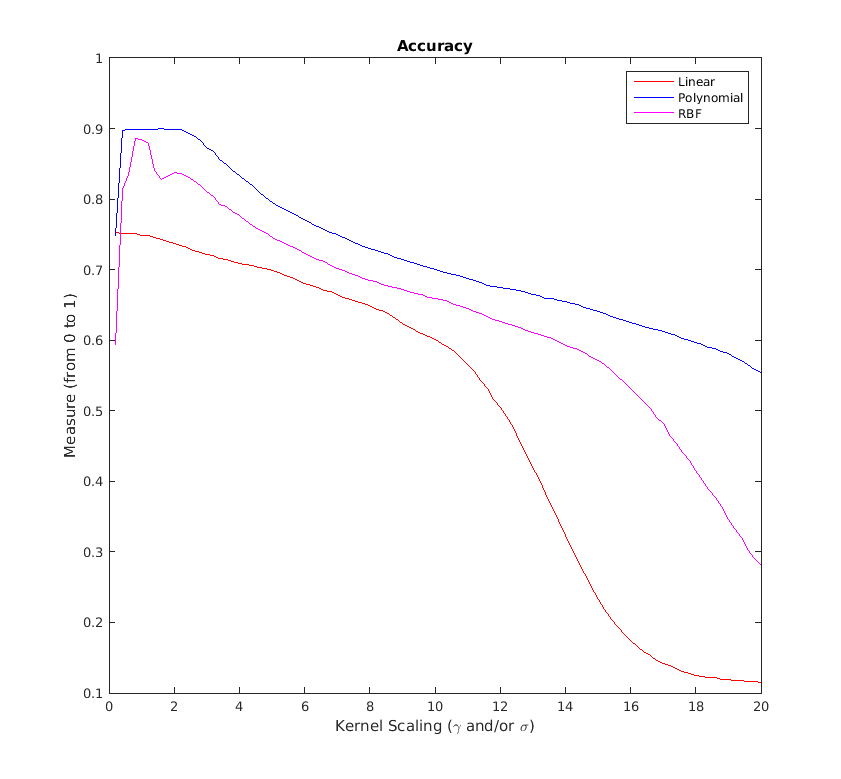
\includegraphics[width=250pt]{images/svm_accuracy.png}}
\caption{Accuracy para cada algoritmo}
\label{img:complete}
\end{figure}

Note-se que os valores de 'accuracy' estão sempre bastante altos para as situações com mais benefícios e para o Kernel Scaling entre 2 e 6 que foram os referidos anteriormente.

\subsubsection{Desenvolvimento - Conclusão}

Existe várias situações que o banco pode optar:
\begin{enumerate}
\item Obter a totalidade de clientes que têm tendência a subscrever a depósitos a termo ('recall' máximo ~0.99), esquecendo a importância de nesses clientes conter alguns que não lhes interessam os depósitos a termo ('precision' muito baixo), o algoritmo que o banco vai usar deve ser SVM com um Kernel polinomial e aumentar o Kernel Scaling até 10, de forma a obter um 'recall' de ~0.99 e um 'precision' de ~0.3. Sendo que o polinomial representa melhores as situações para um valor máximo de 'recall'.
\item Obter a maior parte dos clientes com tendência a subscrever ('recall' bastante alto ~0.9), não esquecendo a importância de não notificar clientes que não estão interessados ('precision' médio ~0.4). Para esta opção é necessário configurar com um SVM do tipo RBF e com um Kernel Scaling de 2 unidades.
\end{enumerate}

Pode-se concluir que SVM cobre bem a situação pretendida pelo banco, no entanto, a taxa de clientes que é atingida em excesso (apesar de acertar nos clientes pretendidos) ainda é bastante alta.

%\bibliography{report} % use a field named url or \url{} for URLs
%\url{www.ua.pt}
% Note: the \bibliographystyle is set automatically

\end{document}
